\section{Projektmanagement}
Wir wollen das Projektmanagement schlank halten um möglichst viel Zeit in die Entwicklung der Artefakte stecken zu können.
Dieser Grundgedanke hat uns bei der im Folgenden beschrieben Auswahl der Modelle und Prozesse geleitet.

% ################################
% Vorgehensmodell
% ################################
\subsection{Vorgehensmodell}

Die Anforderungen an das Vorgehensmodell haben wir folgendermassen definiert:
\begin{itemize}  
\item wenig administrativer Aufwand, schlank
\item passend zur Projektgrösse
\item kompatibel mit den NTB-Vorgaben (Aufteilung Fachmodul, Bachelor-Arbeit)
\end{itemize}

Schnell merkten wir, dass die heutzutage beliebten agilen Vorgehensmodelle wie XP oder Scrum für uns ein Overkill darstellen und aus mehrerer Hinsicht nicht geeignet sind. Bei der Bachelor-Arbeit sind die Anforderungen im Fachmodul-Bericht definiert und ändern sich während der Bachelor-Arbeit nicht mehr. Die zu bearbeitenden Themen-Blöcke weisen untereinander nur sehr wenige Schnittstellen auf und können dadurch als eigenständige Teilprojekte das Modell durchlaufen. Unser Team besteht zudem nur aus zwei Personen, was den Koordinationsaufwand auf ein minimum reduziert.

\begin{figure}[htbp]
	\centering
	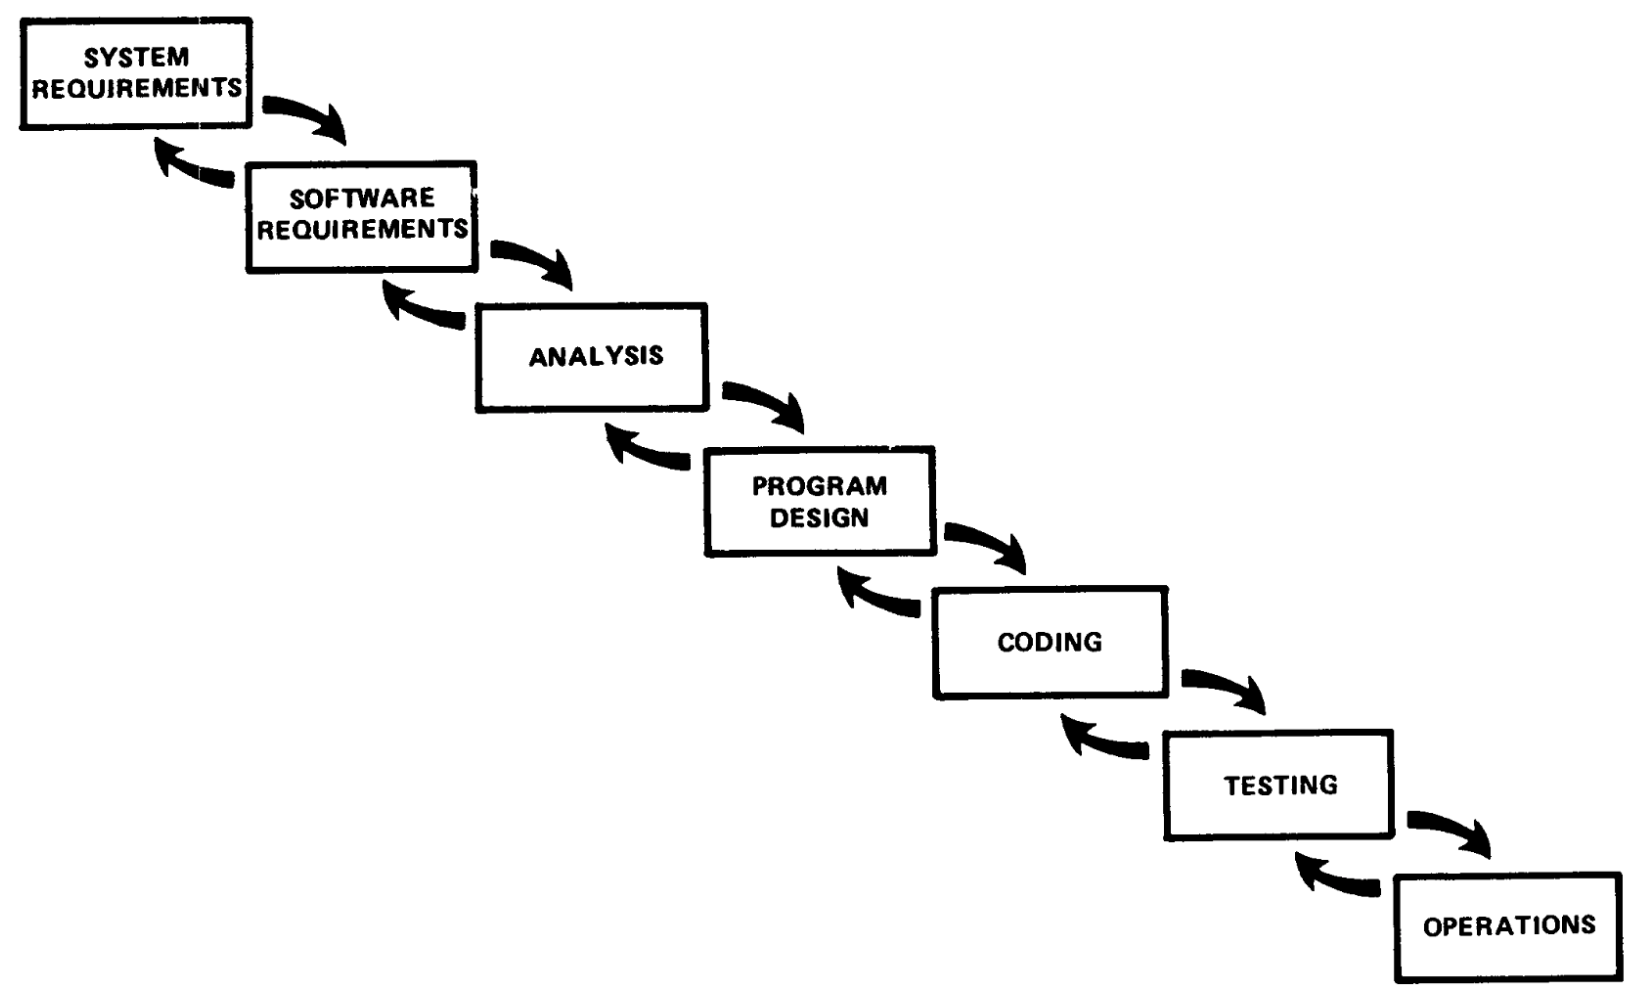
\includegraphics[width=0.9\linewidth]{img/royce-largePrograms}
	\caption{Vorgehensmodell nach Royce}
	\label{img:royce-largePrograms}
\end{figure}


Unsere Bedürfnisse deckt das Vorgehensmodell von Royce ~\cite{Royce1970}, welches in Abbildung  \ref{img:royce-largePrograms} dargestellt ist, am besten ab. Es besteht grundsätzlich aus einem sequentiellen Ablauf der Entwicklungsphasen, berücksichtigt dabei aber auch die Notwendigkeit von Rücksprüngen zur vorherigen Phase.
Die ersten Phasen von der Definition der \textit{System Requirements} bis zu den ersten Gedanken zum Thema \textit{Program Design} behandeln wir im Fachmodul. Der zweite Teil mit der genauen Definition des \textit{Programm Designs} bis zum Betrieb der Software findet anschliessend während der Bachelor-Arbeitszeit statt.


% ################################
% Entwicklungsprozess
% ################################
\subsection{Entwicklungsprozess}
Den Entwicklungsprozess führen wir mit Kanban. Kanban basiert auf dem Pull-Prinzip d.h. jeder, der im Projekt arbeitet, holt sich selbst einen neuen Arbeitsauftrag, sobald er mit einem fertig ist. Die führt dazu, dass die Arbeiten speditiver abgewickelt werden und spart zudem die Stelle des Projektmanagers, der die Aufgaben verteilt.

\begin{figure}[htbp]
	\centering
	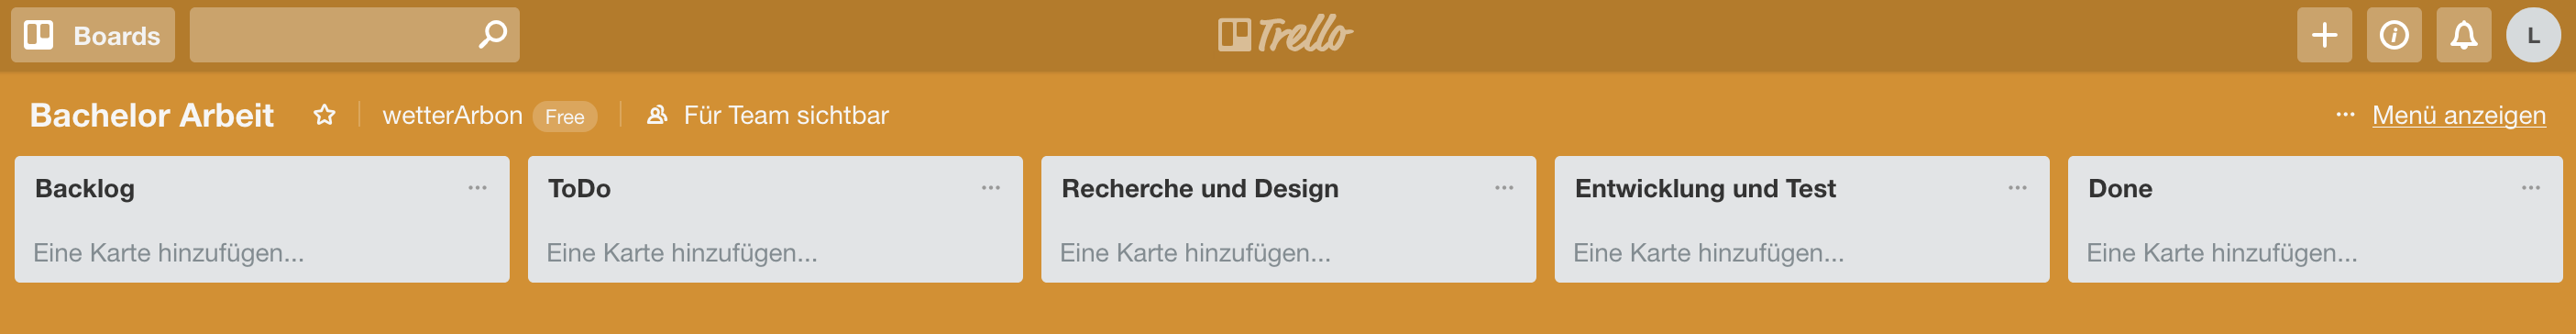
\includegraphics[width=1\linewidth]{img/kanban}
	\caption{Kanban}
	\label{img:kanban}
\end{figure}


David Anderson \cite{AndersonDavidJ2011K:eC} hat das System Kanban, welches ursprünglich aus der Industrie kommt, auf die IT angepasst und dadurch das \textit{Virtuelle Kanban System} entwickelt. Die grundlegenden Regeln daraus lauten:

\begin{itemize}  
\item Jede Karte ist eine Aufgabe
\item Die Aufgabe soll maximal 8 bis16~h benötigen
\item Pro Arbeits-Spalte sind die Anzahl Karten limitiert
\item Eine neue Karte darf erst gezogen werden, wenn die vorherige fertig ist (Multitasking-Vermeidung)
\end{itemize}

% ################################
% Risikoanalyse
% ################################
\subsection{Risikoanalyse}
Für die Risikoanalyse haben wir eine Liste der möglichen  Risiken erstellt. Als Grundlage verwendeten wir das Risikolexikon aus dem Buch \flqq IT-Risikomanagment leben!\frqq ~\cite{AhrendtsFabian2008Il:w}. 
Für jedes Risiko haben wir die Eintretenswahrscheinlichkeit und das Ausmass abgeschätzt. Gegenüber den herkömmlichen Risikobeurteilungen, haben wir allerdings die Auswirkungen auf Kosten und Terminverzug weggelassen, da sie in unserem Projekt nicht relevant sind und uns auf den Stundenaufwand und den Funktionsumfang beschränkt. Um die Auswirkung der einzelen Risiken abschätzen zu können, haben wir eine Punkteskala mit entsprechenden Kriterien erstellt, wie in Tabelle \ref{tab:auswirkung} aufgeführt. \vspace{5mm} %5mm vertical space

\begin{table}[h!]
\centering
\label{tab:auswirkung}
\begin{tabular}{rl}
Wert	[-]	& 	Auswirkung bezüglich Umfang \\
\hline
10	&	Gesamter Block nicht funktionsfähig \\
8	&	Einzelne Funktion nicht umgesetzt  \\
6	&	Bemerkbar, keine Funktionseinbusse \\
4	&	von eingeschränkter Benutzergruppe bemerkbar \\
2	&	von Kunden nicht bemerkbar
\end{tabular}
\end{table}

Die Risikomatrix in Abbildung \ref{img:risikomatrix} zeigt auf grafische Weise wie kritisch die einzelnen Risiken aus der Risikoliste sind. Mindestens vier davon sind als hoch eingestuft und müssen im Rahmen der Bachelor-Arbeit reduziert werden. Dies sind:

\begin{itemize}  
\item Komplexe Datenmigration
\item Mangel an Echtzeitverhalten
\item Mangelnde Ressourcenverfügbarkeit
\item Mangelnde Anforderungsqualität
\end{itemize}


% Abbildung der Risikomatrix
\begin{figure}[h!]
	\centering
	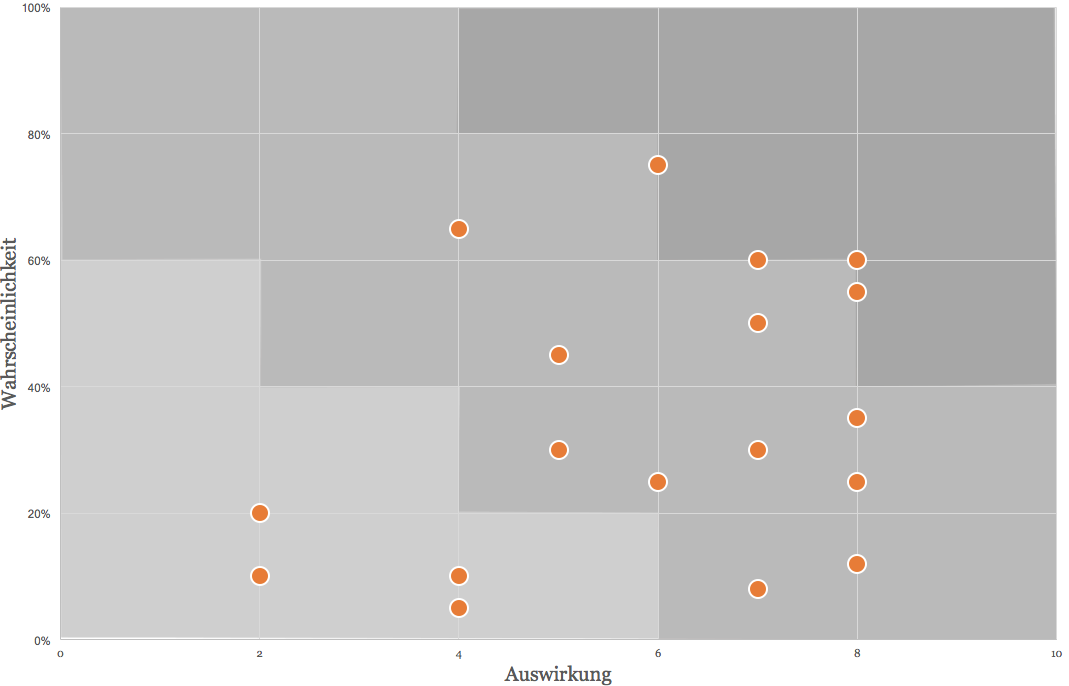
\includegraphics[width=1\linewidth]{img/risikomatrix.pdf} 
	\caption{Risikomatrix}
	\label{img:risikomatrix}
\end{figure}



% ################################
% Projektplan
% ################################

\subsection{Projektplan für die Bachelor-Arbeit}
Der Zeitplan für die Bachelor-Arbeit ist in Abbildung \ref{img:terminplan} auf Seite \pageref{img:terminplan} dargestellt.
Im oberen Teil sind die allgemeinen Termine und Abwesenheiten aufgeführt. Der mittlere Teil zeigt die Arbeitsverteilung über das Semester und am Schluss kommen die Zeitaufwände für Doku und Meetings. Die Dokumentation wollen wir kontinuierlich erstellen, sodass wöchentlich ein entsprechender Block vorgesehen ist.

\begin{figure}[h!]
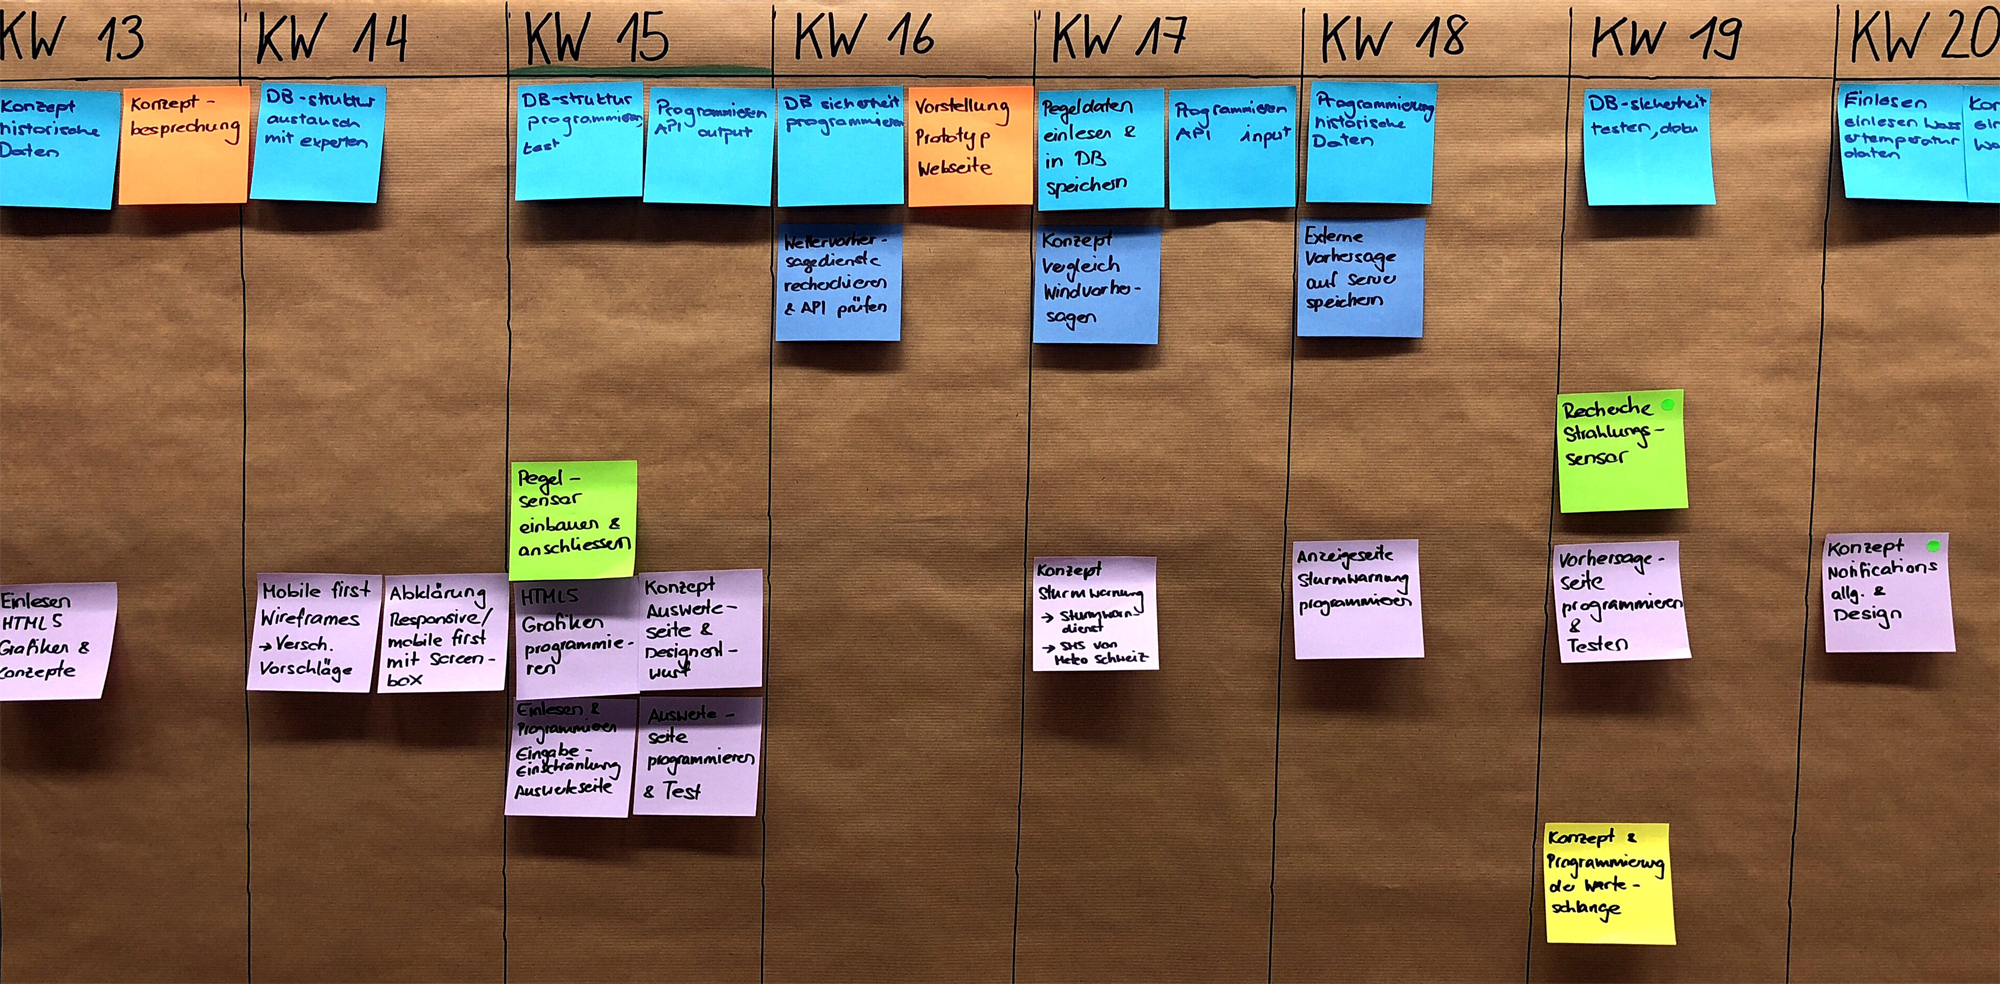
\includegraphics[angle=90,height=1\textheight,keepaspectratio]{img/terminplan.pdf}
\caption{Projektplan für die Bachelor-Arbeit}
\label{img:terminplan}
\end{figure}



